\documentclass[a4paper,11pt]{article}
\usepackage[utf8]{inputenc}
\usepackage[T1]{fontenc}
\usepackage{amsmath}
\usepackage{mathtools}
\usepackage{amsfonts}
\usepackage{amssymb}
\usepackage{graphicx}
\usepackage{multicol}
\usepackage{array}
\usepackage{float}
\usepackage{epstopdf}
\usepackage{caption}
\usepackage{subcaption}
\usepackage{gensymb}
\usepackage[bottom]{footmisc}
\usepackage{appendix}
\usepackage{pdfpages}
\usepackage{todonotes}
\usepackage{mathpazo}
\usepackage{titleps}
\usepackage{color}
\usepackage{xcolor}
\usepackage{colortbl}
\usepackage{siunitx}
\usepackage{pdflscape}
\usepackage{cancel}

\usepackage[skins]{tcolorbox}
\usepackage{sectsty}
\usepackage[arrowmos]{circuitikz}
\usepackage{pgfplots}
\usepackage{blindtext}
\usepackage[inner=2cm,outer=2cm,top=2.5cm,bottom=2.5cm]{geometry}
\usepackage{todonotes}
\usepackage{hyperref}
\usepackage{url}
\usepackage{adjustbox}
\usepackage{tabularx}
\usepackage{booktabs}
\usepackage{fancybox}
\usepackage[tikz]{bclogo}



%For code insertion
%listing
\usepackage{listings}
\usepackage{xcolor}
\definecolor{codegreen}{rgb}{0,0.6,0}
\definecolor{codegray}{rgb}{0.5,0.5,0.5}
\definecolor{codepurple}{rgb}{0.58,0,0.82}
\definecolor{backcolour}{rgb}{0.98,0.98,0.98}
\lstdefinestyle{mystyle}{
    backgroundcolor=\color{backcolour},
    commentstyle=\color{codegreen},
    keywordstyle=\color{blue},
    numberstyle=\tiny\color{codegray},
    stringstyle=\color{codepurple},
    basicstyle=\ttfamily\footnotesize,
    breakatwhitespace=false,
    breaklines=true,
    captionpos=b,
    keepspaces=true,
    numbers=left,
    numbersep=5pt,
    showspaces=false,
    showstringspaces=false,
    showtabs=false,
    tabsize=2
}
\lstset{style=mystyle}



\graphicspath{{figures/}}
\sectionfont{\large}
\subsectionfont{\normalsize}



%%%%%%%%%%%%%%%%%%%
% HANDS-ON NUMBER
\newcommand\handsOnN{FPGA}
%%%%%%%%%%%%%%%%%%%

\newpagestyle{main}{
	\sethead[LELEC2102][][]{LELEC2102}{}{}
	\headrule
    \setfoot[][\thepage][]{}{\thepage}{}
}

\newcommand{\horrule}[1]{\rule{\linewidth}{#1}} % Create horizontal rule command with 1 argument of height
%\setlength {\marginparwidth }{2cm}
%%%%%%%%%%%%%%%%%%%%%%%%%%%%%%%%%%%%%%%%%%%%%%%%%%%%%%%%%%%%%%%%%%%%%%%%%%%%

\begin{document}
\renewcommand{\figurename}{Fig.}

\renewcommand{\thepage}{\arabic{page}}
\setcounter{page}{1}
\pagestyle{main}
\newpage \clearpage

\begin{center}
\begin{LARGE}
LELEC2102: Hands-on FPGA
\end{LARGE}
\vspace{0.3cm}
%\textit{TA 1, TA 2}
\end{center}

\section*{Introduction}

In this Hands-On, you will be introduced to the basics of microcontroller unit (MCU) operation and interrupt-based embedded programming. We will use so-called bare metal programming, which means we will not use an operating system: you will be in control of all the code that runs on the device! As this is most likely your first project dealing with bare metal embedded programming, we will provide you with a functional baseline code to start with. Then, you will be guided step by step to develop the key skills needed for this part of the project.
\begin{bclogo}[couleur = gray!20, arrondi = 0.2, logo=\bcinfo]{Explanation of the hands-on boxes}
In this note, there are a few boxes presenting additional information:
\begin{itemize}
    \item \bcinfo will provide you some more detailed explanations.
    \item \bcattention will explain typical mistakes that might lead to errors or a non functional system.
    \item \bcquestion will provide you with additional questions or experiments that will improve your understanding of the system. We advise you to leave them for the end of the hands-on as they are not critical.
\end{itemize}
\end{bclogo}

\section*{Objectives}

\begin{itemize}
    \item Learn how to use GNU Radio to demodulate packets transmitted by the S2LP radio.
    \item Understand how a SDR receiver works.
\end{itemize}

%\section*{Material \& preparation}

\begin{comment}[couleur = gray!20, arrondi = 0.2, logo=\bcinfo]{}
\vspace{0.2cm}
\end{comment}
For this hands-on session, you will need:
\begin{itemize}
    \item The Nucleo MCU board with its sensing and power-management board ;
    \item A USB cable to connect your computer to the Nucleo;
    \item A LimeSDR connected to the MCU with a SMA cable.
\end{itemize}

\section{Accelerating the detection of the preamble}
In the previous Hands-On, our demodulation chain required a component called the \textit{preamble detector} that actively seeks the preamble sequence located at the beginning of a packet by looking at the energy of each sample and accumulating it over time. When the accumulated value exceeded a threshold, the preamble was considered present and a given amount of samples were forwarded to the synchronization stage. This system allows to avoid unnecessary heavy computations as well as real-time operation. There are two drawbacks to this process. First, the threshold is not updated and increasing the gain of the RF front-end will increase the noise power, possibly going above the set threshold. Second, this preamble detection scheme requires a lot of computation, calculating and accumulating the energy of each sample. \\

As it operates continuously, it is best to move its functionality from software towards a specialized piece of hardware in order to improve its \textbf{energy efficiency and processing speed}. If we decide at one point to increase the packet rate of the overall transmission chain, this solution is more robust regarding packet misses. It is also further motivated by the fact that this block occurs at the very beginning of the processing chain, just after the low-pass filter. We will also change the behavior of the block by calculating the threshold based on the noise power and on a programmable margin coefficient. The accelerated block will therefore be called the packet presence detector (PPD). However, we only want to accelerate the energy detection step but still receive all samples in GNU Radio to be able to monitor the channel if needed. Therefore, the PPD will add a flag at the start of a packet when it has been detected. This flag corresponds to the value \texttt{0x7FF} which can not be practically reached by the LMS7002M chip.


\subsection{Design overview}
We implemented for you a packet presence detection module in SystemVerilog HDL\footnote{Although uncommon, it is possible to mix multiple HDL languages in a single design. For instance, the majority of the LimeSDR-Mini system is written in VHDL, but for your convenience we have written the PPD in SystemVerilog.}. First, open the Quartus project, \texttt{LimeSDR-Mini\_lms7\_lelec210x/LimeSDR-Mini\_lms7\_lelec210x.qpf}. If a message asking you for overwriting the database is printed, click "yes". With Quartus or any other code editor, you can then open the PPD design file located in\\ \texttt{LimeSDR-Mini\_lms7\_lelec210x/ip/packet\_presence\_detection/packet\_presence\_detection.sv}\\ and containing the following interfaces:
\begin{itemize}
    \item A clock and reset interface.
    \item A sink (input) streaming interface with data and valid signals.
    \item A source (output) streaming interface with data and valid signals.
    \item A custom static interface for configuration signals.
\end{itemize}
The PPD follows the low-pass filter in the receiver chain, as you have seen in previous hands-on. The filter, implemented using a FIR, is already included in the hardware design provided to you. Indeed, as a FIR is composed of multiply-and-accumulate operations, it can be easily accelerated in hardware. The  PPD module is integrated as a custom IP inside the same subsystem as the FIR, it therefore shares the same streaming interfaces\footnote{See pp 40-52 of \texttt{mnl\_avalon\_spec.pdf} on Moodle for details.}: the data bus is 24-bit wide with the MSBs and LSBs containing the samples of the I and Q channels respectively. In addition a valid signal is associated with the streaming data to indicate whether the data bus contains information of interest, or not. With the PPD, the goal is to produce an output valid signal that indicates if the complex magnitude of the data has reached a threshold.

\begin{figure}[h]
    \centering
    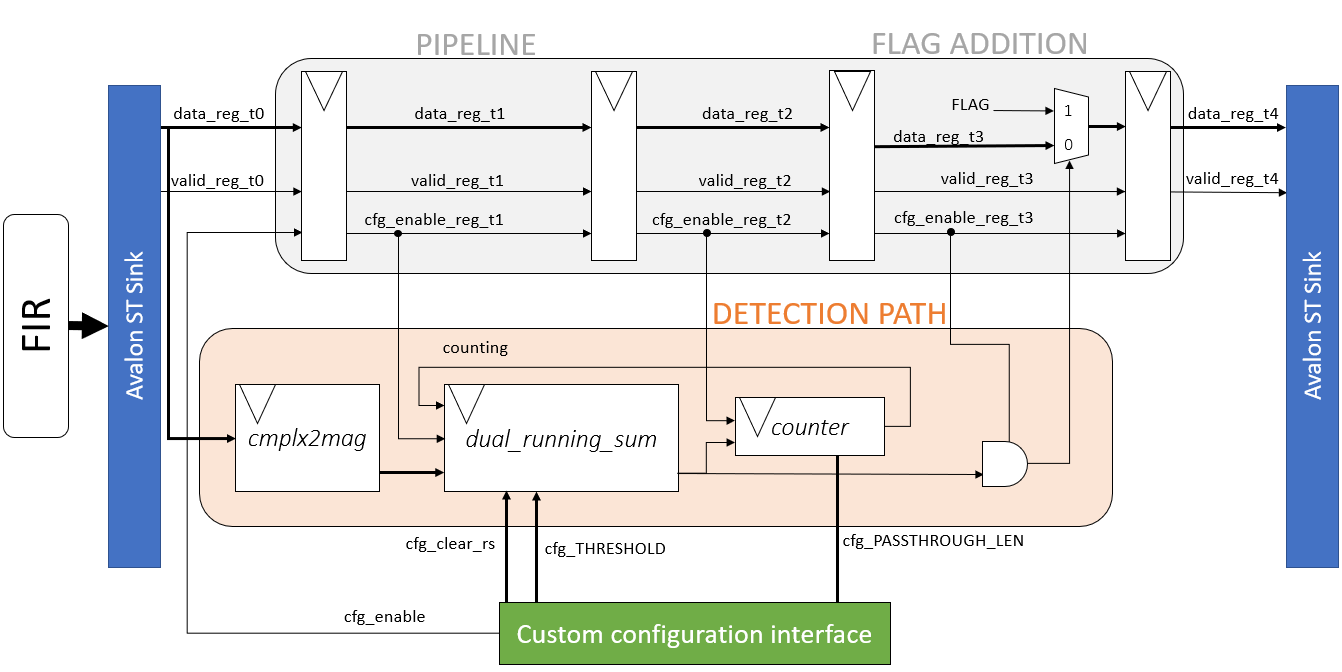
\includegraphics[width=\linewidth]{figures/packet_presence_detection.png}
    \caption{Hardware packet presence detector schematic}
    \label{fig:pd_schematic}
\end{figure}

\subsection{Packet presence detector schematic}
In Figure \ref{fig:pd_schematic} below you can find a schematic of the different modules that compose the PPD. As a reminder, the objective of this block is to add a flag at the start of a packet when a sufficient energy has been detected in the signal. It functions as follows:
\begin{enumerate}
    \item \textbf{Complex to magnitude: } The IQ samples are processed by a \textit{complex to magnitude} block which outputs the magnitude of the complex IQ vector.
    To do so, we calculate the magnitude as the square root of $I^2+Q^2$. As square-root function are difficult to implement in hardware logic, we are thus going to use a very simple and accurate algorithm. The estimate for the first quadrant of the trigonometric circle is drawn on Figure \ref{fig:cmplx2mag}. The mathematical formula is provided to you in Equation \ref{eq:1norm}\footnote{Further information can be found online: \url{https://en.wikipedia.org/wiki/Alpha_max_plus_beta_min_algorithm} and \url{http://dspguru.com/dsp/tricks/magnitude-estimator/}.}.

    \begin{equation}
        |z| = \frac{min(|I|,|Q|)}{4} + max(|I|,|Q|)
        \label{eq:1norm}
    \end{equation}

    \begin{figure}[h]
        \centering
        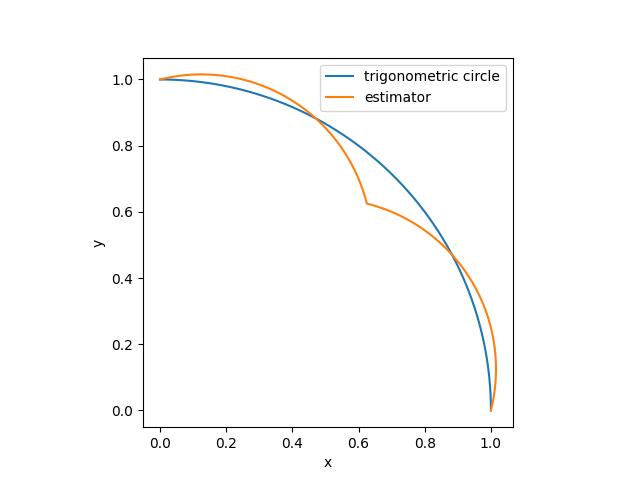
\includegraphics[width=0.45\linewidth]{figures/trigo.png}
        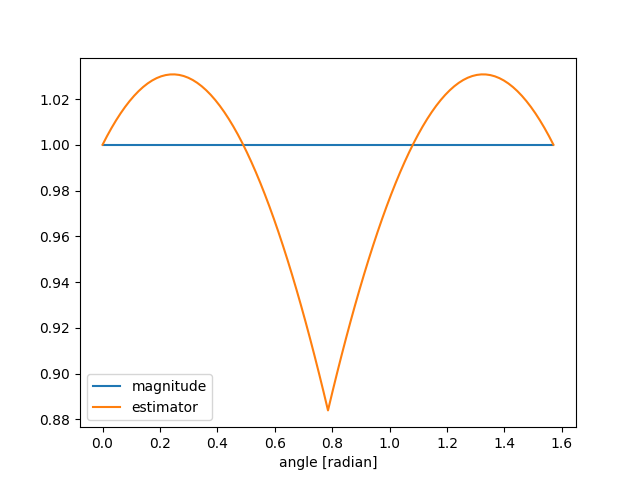
\includegraphics[width=0.45\linewidth]{figures/angle.png}
        \caption{Complex Magnitude Estimator output in x-y coordinates (left) or polar coordinates (right) for input points of the trigonometric circle.}
        \label{fig:cmplx2mag}
    \end{figure}

    \item \textbf{Dual running sum: } The estimated complex magnitude of the samples is then averaged over multiple samples by two moving average filter of different length in series, a short-term sum and long-term one. They are implemented by forwarding input samples in  memory-based \textit{delay lines}, developped by Altera.

    \begin{align}
            y[n] = \sum_{k=0}^{N-1}\left|x[n-k]\right|
    \end{align}

    At each clock cycle an accumulator adds and substracts the first and last magnitude values stored in the delay line to its content. This structure is more efficient than the general FIR because we know each tap is equal to one, we therefore only need two adders.

    \begin{align}
            y[n+1] = y[n] + \left|x[n]\right| - \left|x[n-N+1]\right|
    \end{align}

    The two moving average filters have two different functions. The first one, the short-term sum, receives the sample magnitudes first and its delayed output value are then forwarded to the long-term sum. This longer delay line is used to evaluate the noise power.

    \begin{figure}[h]
        \centering
        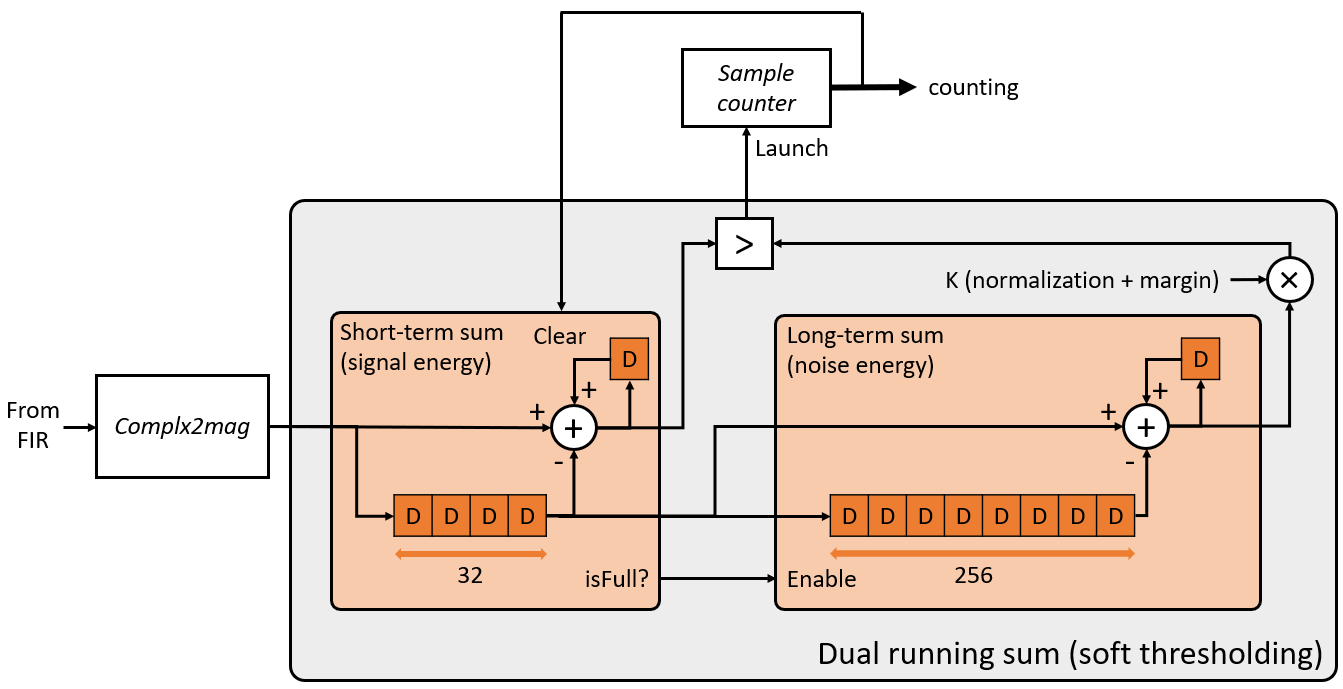
\includegraphics[width=\linewidth]{figures/dual_running_sum_block.png}
        \caption{Architecture of the dual running sum}
        \label{fig:dual_runnign_sum}
    \end{figure}

    The overall architecture of the dual running sum is shown in Fig. \ref{fig:dual_runnign_sum}. If no packet is being received, the samples contain only noise. They pass through the short-term sum and then the long-term one. Both their accumulator can then be seen as noise power estimations.  When a packet arrives, possibly with  higher energy than the noise, the corresponding samples first enter the short-term sum. Its accumulator value therefore increases and might at one point exceed the accumulator value of the long-term sum, which contains only noise samples. At this point, a packet is considered present and a launch signal is triggered.

    To be noted, when a packet is detected and the counter (next block) is enabled, we clear the short-term sum and disable the long-term one, to avoid any retriggering or corruption of our noise evaluation by packet samples.


    \item \textbf{Counter :} This block receives the launch signal of the previous block. This counter block is used to count the samples when the threshold has been reached and avoid triggering a start flag multiple times inside a single packet. During the sequence, a \texttt{running} signal indicates the state of the counter. This signal is used to clear the short-term sum of the dual running sum. The number of samples that are passed is configurable.

    \item \textbf{Flag addition :} A multiplexer is used at the end to replac a sample with a flag, here $I=$\texttt{0x7FF} and $Q=$\texttt{0x7FF}, when the launch signal is triggered.

\end{enumerate}


In order to reduce the length of the critical path between registers, we use a paradigm called \textit{pipelining}. In short, we divide the operations of the PPD into several stages with similar length. As the critical path in this configuration is much shorter, it allows to operate the circuit at a higher frequency. In return, the additional registers add area and energy consumption to the design. It also requires to forward control signals in the pipeline and it can add complexity (see \textit{Control Path} in Figure \ref{fig:pd_schematic}). You will learn the concept of pipelining in details when studying the \textit{pipelined processor} in the course of \texttt{LELEC2531}.

Try to understand the SystemVerilog implementation of those blocks with respect to their theoretical behavior. Pay particular attention to the bus width of intermediate signals, they are computed in order to systematically avoid any overflow of intermediate values!


\subsection{Modification and simulation of the PPD}


We will first ask you to make some modifications to the dual running sum, more specifically to the comparison between the short- and long-term sum results. In order to make it adaptative from GNU Radio, we will use the \texttt{cfg\_THRESHOLD} signal of the packet presence detection module to multiply the result of the long-term sum before comparing it to the short-term sum result. This allows to be more selective regarding the signal-to-noise ratio required to detect the packet. Increasing its value will limit the risk of false alarm due to noise but make your system less sensitive. In short, with this parameter set to 10, the PPD would require a signal magnitude 10 times higher than the noise one to trigger a detection. However, we should also normalize the short-term and long-term result with respect to the delay line length, the second one being here eight times longer than the first. Overall, we ask you to implement the multiplication shown in Figure \ref{fig:dual_runnign_sum}. In the SystemVerilog code, go to the line 199. We ask you to implement both the normalization, i.e. division by eight, and the multiplication operation on the same line. Note that the \texttt{cfg\_THRESHOLD} signal is connected to the \texttt{K} input of the dual running sum module.


\begin{bclogo}[couleur = gray!20, arrondi = 0.2, logo=\bcquestion]{Division by eight}
    \begin{itemize}
        \item Performing multiplications and divisions is much more complex than simple additions. However, when performing operations with values that are power-of-two, things always seem easier. What would be an efficient way to perform the division by eight?
        \item The order in which the two operations are performed, here the multiplication by K and division by eight, would normally have no importance. Is it the case here? Which operation should be performed first and why?
    \end{itemize}
\end{bclogo}

Once you have implemented this function, we should now test the PPD. We have developped a testbench for you, and we will use ModelSim to verify the PPD behavior before deploying it into the complete system. A few python scripts located at \texttt{ip/packet\_presence\_detection/testbench/python} allow you to generate input vectors for the PPD and compare the testbench output with an expected result obtained with python:

\begin{enumerate}
    \item \texttt{1\_input\_gen.py} : generates input vectors and export them as input vector of the PPD HDL implementation.

    \item To generate the testbench, we will use the \textit{Platform Designer}. It allows the interconnection of multiple blocks of a digital design with a more intuitive user interface. Open the \textit{Platform Design} using the shortcut highlighted in Figure \ref{fig:quartus_platform_designer}. Open the \texttt{packet\_presence\_detection\_tb\_gen.qsys}, and go in \textit{Generate} in the upper left corner, then \textit{Generate Testbench System}. Change the path to \texttt{LimeSDR-Mini\_lms7\_lelec210x/ip/packet\_presence\_detection/} and click on \textit{Generate}. To execute the testbench, open ModelSim and change the working directory to\\ \texttt{ip/packet\_presence\_detection/testbench}. Then run \texttt{do run\_sim.tcl} in order to compile and launch the simulation.

\begin{figure}[H]
    \centering
    
\includegraphics[scale=0.7]{figures/quartus_toolbar.PNG}
    \caption{Toolbar of Quartus. The Platform Designer shortcut is highlighted in yellow.}
    \label{fig:quartus_platform_designer}
\end{figure}

    \item \texttt{2\_compare} : when the SystemVerilog testbench has been executed, compares the input data samples to the output of the PPD, plotting them. Is the PPD working as expected? Do not hesitate to ask your questions to a teaching assistant to ensure you fully understand where and why flags are added.
\end{enumerate}

Once you have analysed the results, we will propagate the changes you made to the complete system that will be flashed on the FPGA. Remember we only modified the IP, we now need to propagate those changes to the actual design. In the \textit{Platform Designer}, open the \texttt{lms\_dsp.qsys} design. Nothing has to be done except clicking \textit{"Generate HDL ..."} on the bottom right of the window and update the path to
\texttt{LimeSDR-Mini\_lms7\_lelec210x/lms\_dsp/} if it is not made automatically. Then press on \textit{"Generate"}. The changes you made locally to the PPD have now been propagated. In the Platform Designer, you can quickly observe the structure of the \textit{lms\_dsp} block, with the FIR, the packet presence detection and the different Avalon Streaming Interface.

You can now compile your design and observe the resource and timing report. Be careful when launching a compilation in Quartus, a window may ask you to update the project revision. Answer \textit{"NO"}.

\begin{bclogo}[couleur = gray!20, arrondi = 0.2, logo=\bcattention]{MAX 10 Device Support might not be installed}
    The support for the FPGA device we use might not be installed in the Quartus you have, which will lead to errors in the compilation. The installation instructions are provided in the wiki of the course.

\end{bclogo}

\subsection{Timing and ressource analysis}

As you have seen in course, an important aspect of digital design is to ensure that your design meet both the resource and timing requirements. Indeed, long combinatorial logic path can lead to setup or hold constraints violations. Now that the design has been compiled, you can check the compilation report using the shortcut highlighted in Figure \ref{fig:compilation_report_button}.

\begin{figure}[h]
    \centering
    
\includegraphics[width=\linewidth]{figures/Compilation_report_button.PNG}
    \caption{Toolbar of Quartus. The Compilation Report shortcut is highlighted in red.}
    \label{fig:compilation_report_button}
\end{figure}


In the \textit{"Flow Summary"} tab, the resource utilisation is reported. Observe for instance the number of embedded multipliers that are employed. Moreover, in the \textit{"Analysis \& Synthesis/Timing Analyzer"} tab, you can see the results for the different corners, constraints violations being highlighted in red. Try to identify the faulty clock involved. In the different summary proposed, you can right click on a clock and select \textit{"Report Timing... (In Timing Analyzer UI)"}. In the opened window, just press \textit{"Report Timing"} at the bottom. Those steps are depicted in Figure \ref{fig:report_timing_analyzer}. You can now analyze the most critical path implying the selected clock, as well as the logic cells involved. Try to link the critical path to the RTL design. It should involve a signal starting in the dual running sum module. An easy fix is here to add a register in the path to break in two. This will delay the launch signal by one clock cycle, which is not problematic. \textbf{If you make a modification to the verilog of the PPD, you need to regenerate it in the Platform Designer}.

\begin{figure}[h]
    \centering
    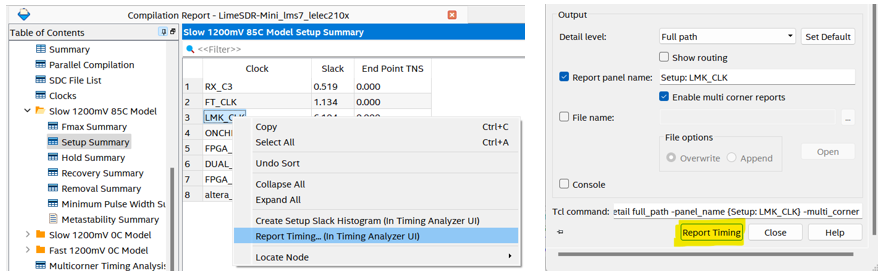
\includegraphics[width=\linewidth]{figures/Report_Timing_Analyzer.png}
    \caption{Steps to analyze the most critical path on a given clock.}
    \label{fig:report_timing_analyzer}
\end{figure}

Moreover, we prevented \textbf{register retiming} which allows the synthesis tool to balance the combinatorial logic across registers when it does not affect the system behaviour. This helps on meeting the timing requirements by offloading parts of long combinatorial path. To enable this setting, go in \textit{"Assignments/Settings/Compiler Settings"} on Quartus and uncheck the \textit{"Prevent register retiming"} box.

Before relaunching a compilation, ask for an assistant to check your modifications, to avoid wasting precious synthesis time. Done? Now relaunch a compilation and analyze the results. Again, if a window asks you to update the project revision, answer \textit{"NO"}. Is there still a timing constraint violation? Can you still link the most critical path to the HDL design?

To analyse the ressource used by the design, you can look at the \textit{Hierarchy} tab in the \textit{Project Navigator}. More than navigating through the design, you can also look at the ressource used by each module. Analyse the resource usage of the PPD, more specifically the memory bits and the DSP.
\begin{comment}
\subsection{From Euclidean norm to Absolute-value norm}

In order to meet the timing requirements, another solution is to use a less complex estimation of the IQ samples magnitude. We are thus going to use a very simple and accurate algorithm that does not have the burden of implementing the complex logic of \textit{integer multiplication}. The estimate for the first quadrant of the trigonometric circle is drawn on Figure \ref{fig:cmplx2mag}. We ask you to implement it in System Verilog, the mathematical formula being provided to you in Equation \ref{eq:1norm}\footnote{Further information can be found online: \url{https://en.wikipedia.org/wiki/Alpha_max_plus_beta_min_algorithm} and \url{http://dspguru.com/dsp/tricks/magnitude-estimator/}.}. Your modification of the \texttt{cmplx2mag} module must be done in the \texttt{USER CODE} parts, which goes from line 45 to 52 and on line 210. As we were performing two multiplications and one addition in the previous algorithm ($I^2+Q^2$), the data bus at the output of the \textit{cmplx2mag} module was specified as twice the input data bit width (due to multiplication) plus one (due to the addition). This is specified on line 210, do not forget to adapt it for the new algorithm. In the next step, you are going to make a behavioral simulation of you implementation to validate it.

\begin{equation}
    |z| = \frac{min(|I|,|Q|)}{4} + max(|I|,|Q|)
    \label{eq:1norm}
\end{equation}

\begin{figure}[h]
    \centering
    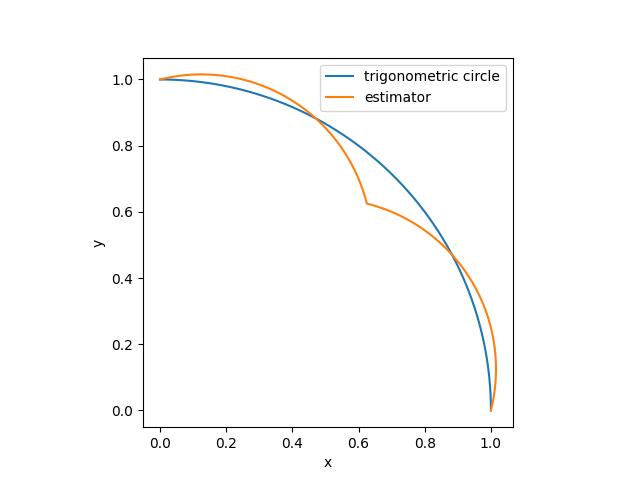
\includegraphics[width=0.45\linewidth]{figures/trigo.png}
    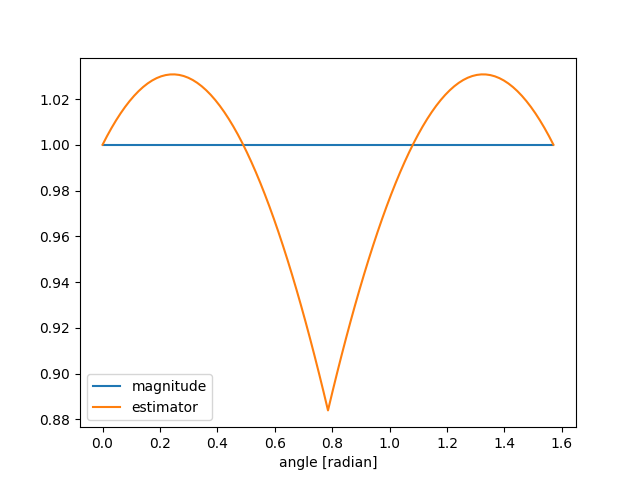
\includegraphics[width=0.45\linewidth]{figures/angle.png}
    \caption{Complex Magnitude Estimator output in x-y coordinates (left) or polar coordinates (right) for input points of the trigonometric circle.}
    \label{fig:cmplx2mag}
\end{figure}


Now that you have a functional design for the PPD with the Absolute-value norm, we can perform a synthesis of the complete design. Do not forget to propagate your change by regenerating the HDL via the Platform Designer. Observe the resource usage and the timing report, is there still a timing constraint violation?

\end{comment}


\section{Packet formatting}

The transmitted packets shall have the following format
\begin{center}
\texttt{r$\mathbin\Vert$emitter\_id$\mathbin\Vert$payload\_length$\mathbin\Vert$packet\_serial$\mathbin\Vert$app\_data$\mathbin\Vert$tag}
\end{center}
(\texttt{$\mathbin\Vert$} denotes concatenation)
where
\begin{center}
\begin{tabular}{lccl}
    Field & Length (bytes) & Encoding & Description \\ \hline
    \texttt{r} & 1 & & Reserved, set to 0.\\
    \texttt{emitter\_id} & 1 & BE & Unique id of the sensor node.\\
    \texttt{payload\_length} & 2 & BE & Length of \texttt{app\_data} (in bytes).\\
    \texttt{packet\_serial} & 4 & BE & Unique and incrementing id of the packet. \\
    \texttt{app\_data} & any  &  & The feature vectors. \\
    \texttt{tag} & 16 & & Message authentication code (MAC). \\
\end{tabular}
\end{center}

\begin{bclogo}[couleur = gray!20, arrondi = 0.2, logo=\bcquestion]{Reserved byte}
    What could be the purpose of a ``reserved'' byte ?
\end{bclogo}
\begin{bclogo}[couleur = gray!20, arrondi = 0.2, logo=\bcinfo]{Endiannes}
    As you can see, a packet is defined as a sequence of bytes and is formed by
    the concatenation of multiple fields.
    Some of those fields are integers that are encoded on multiple bytes (since
    encoding e.g. a 32-bit integer on a single byte is not possible) and we
    therefore need to specify the encoding, that is, the mapping between the
    number and the byte sequence.
    For unsigned fixed-size integers, there are two very common byte encoding:
    little endian (LE) and big endian (BE).
    Let us take the example of a 32-bit unsigned integer, that is a number $x \in
    \{0,\dots, 2^{32}-1\}$.
    Let $x_0,x_1,x_2,x_3\in\{0,...,255\}$ be such that $x = \sum_{i=0}^3 x_i 256^i$.
    The LE encoding of $x$ is \texttt{$x_0$$\mathbin\Vert$$x_1$$\mathbin\Vert$$x_2$$\mathbin\Vert$$x_3$} (the least
    significant byte comes first) while its BE encoding is
    \texttt{$x_3$$\mathbin\Vert$$x_2$$\mathbin\Vert$$x_1$$\mathbin\Vert$$x_0$}.  (the most significant byte comes
    first).
    The LE/BE encodings work similarly for encoding 16-bit (resp. 64-bit,
    128-bit\dots) numbers on 2 (resp. 8, 16\dots) bytes.
    For 8-bit numbers encoded on one byte, the BE and LE encodings are identical.
\end{bclogo}

\begin{bclogo}[couleur = gray!20, arrondi = 0.2, logo=\bcinfo]{Features encoding}
    The feature vectors are a list of MEL vectors (ordered by acquisition
    time), and each MEL vector is a list of 16-bit numbers (ordered from lower
    to higher frequency band).
    The \texttt{app\_data} contains sequentially the MEL vectors, and the
    encoding of each MEL vector is the concatenation (respecting the order) of
    the encoding of the numbers it is made of.  The numbers are encoded on
    2~bytes, in BE.
    You do not need to implement this (it is already done in the \verb|encode_packet| function).
\end{bclogo}

As for each hands-on, start by synchronizing your Git. In the MCU code, the function in charge of forming the packet is
\verb|make_packet| in \texttt{packet.c}.
Its prototype is:
\begin{lstlisting}[style=customc]
int make_packet(uint8_t *packet, size_t payload_len, uint8_t sender_id, uint32_t serial);
\end{lstlisting}
This function takes as input \texttt{packet}, a buffer of bytes of length
\texttt{PACKET\_HEADER\_LENGTH + payload\_len + PACKET\_TAG\_LENGTH}, in
which \texttt{app\_data} should already have been written starting at byte\\
\verb|packet[PACKET_HEADER_LENGTH]|.
The function has to write the remaining parts of the packet (the header and the tag) in the buffer and return the total length of the packet.

\textbf{
    Implement \texttt{make\_packet}, except for the \texttt{tag} part of the
    packet, which is already set by an incorrect function that we will work on afterwards.
    Check that your implementation does not trigger any compiler warning, then
    check that the packet are now decoded correctly on your PC. Be aware that the \texttt{app\_data} data field is already included in the packet\footnote{You can take a look at the method \texttt{encode\_packet} in \texttt{adc\_dblbuf.c} to see how it is done.}.
}

\section{Message authentication code}

Let us now consider the authentication of the message. The authentication
\texttt{tag} is defined as
\[
    \texttt{tag} = \text{CBC-MAC-AES}_{k}\left(
        \texttt{r$\mathbin\Vert$emitter\_id$\mathbin\Vert$payload\_length$\mathbin\Vert$packet\_serial$\mathbin\Vert$app\_data}
    \right)\;,
\]
where $k$ is a secret key (an sequence of 16 bytes) shared between the sensor
node and the receiver. This secret key should be uniformly random. The $\text{CBC-MAC-AES}$ algorithm is described in \autoref{algo:cbc-mac-aes} and its block diagram is shown in \autoref{fig:cbc-mac-aes}.

\begin{bclogo}[couleur = gray!20, arrondi = 0.2, logo=\bcquestion]{What does an authentication tag do ?}
    You have had a quick introduction to the authentication basic knowledge in Lecture L3b.\\
    Based on that and on the description of the message authentication code, what is your understanding of the purpose of the authentication tag ? What does it prevent or allow ?\\
    More importantly, what \textit{doesn't} it prevent ? Is the header readable or encrypted ? And the message data ?
\end{bclogo}

\begin{algorithm}
\begin{algorithmic}
    \REQUIRE Message $x$ (sequence of bytes) to authenticate.
    \REQUIRE Secret key $k$ (sequence of 16 bytes)
    \ENSURE The authentication tag $t$ (sequence of 16 bytes).
    \STATE Parse $x$ into blocks $\left(x_1,x_2,\dots,x_n\right)$ such that the
    length of each block is 16 bytes (except for $x_n$).
    \STATE If the length of $x_n$ is not 16, append as many zero bytes to $x_n$
    to extend it to 16 bytes.
    \STATE $s \leftarrow 0^{16}$ (Where $0^{16}$ denotes the string made of 16 zero bytes.)
    \FOR{$i=1\dots,n$}
    \STATE $s \leftarrow \text{AES}_k(s \oplus x_i)$
    \ENDFOR
    \STATE $t \leftarrow s$
\end{algorithmic}
\caption{CBC-MAC-AES}
\label{algo:cbc-mac-aes}
\end{algorithm}

\begin{figure}[h]
\centering
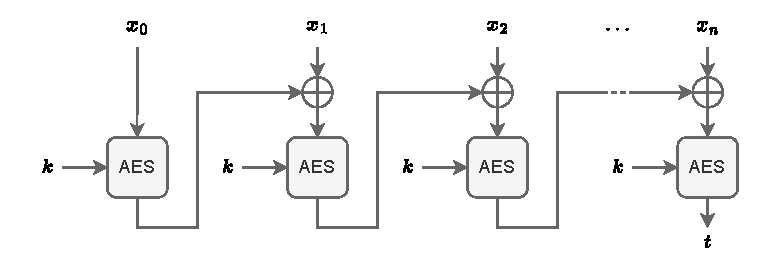
\includegraphics[scale=1]{figures/crypto_cbc_mac_aes.pdf}
\caption{Block diagram of CBC-MAC-AES}
\label{fig:cbc-mac-aes}
\end{figure}

You have to complete the function \texttt{tag\_cbc\_mac()}, which is already present in the \texttt{packet.c} file, by implementing the CBC-MAC-AES algorithm with the following constraints: the function \textbf{must not allocate memory}, and its stack space usage must be constant (i.e., independent of the message length).
We provide you the AES reference implementation (\texttt{aes\_ref.h}), whose
prototype is the following:
\begin{lstlisting}[style=customc]
void AES128_encrypt(unsigned char* block, const unsigned char* key);
\end{lstlisting}
where \texttt{block} is both the input and output of the AES block cipher (it
is modified in-place).
Both \texttt{block} and \texttt{key} are expected to point to 16-byte buffers. Regarding the key, you can modify and use the \texttt{AES\_Key} variable defined on top of the file.

\textbf{
    First, re-write the CBC-MAC-AES algorithm to make it easier to
    implement with the given constraints. Once your have the pseudo-code, translate it in C. Check that your implementation does not trigger any compiler warning.
}

If there are no errors, we are now going to compile and launch the whole MCU application for the project. To do so, go in the \texttt{config.h} file and change the \texttt{RUN\_CONFIG} from \texttt{EVAL\_RADIO} to \texttt{MAIN\_APP}. You can now recompile the design and flash it on the MCU. Launch the GNU Radio \texttt{main\_app} (do not forget to change the carrier frequency). To authenticate the packets, you need to launch a script. To do so, refer to the \texttt{README} of the \texttt{auth} subdirectory.

\section{Performance characterization}
At the end of the semester, you will have to characterize your system. Regarding the MCU, you might want to have an insight on the number of cycle of a given task, as well as the code size. Here are a few tools you can use to extract such information. In order to verify the performance of an implementation, one needs to measure it's key metrics, namely the cycle count, and the code size. We provide you here with explanations on how to make these measurements. Additionally, when compiling, several optimizations steps are provided by the compiler. Those are grouped into optimization levels for ease of use. Follow the explanations in the corresponding box to change the optimization levels.


\begin{bclogo}[couleur = gray!20, arrondi = 0.2, logo=\bcinfo]{How to measure cycle counts} In order to measure the time taken by an implementation, the most basic way is to use a time measuring device, however, this is not precise enough as the MCU can execute several millions of cycles every second. A more accurate method is to measure the number of cycles taken by the CPU. To do so, you will need a special register that is a cycle counter. For ARM processors, if a cycle counter is present, the two registers of interest are :
\begin{lstlisting}[style=customc]
DWT->CTRL |= 1 ; // enable the counter
DWT->CYCCNT = 0; // reset the counter
\end{lstlisting}
After your implementation has run, you can read the value contained in \texttt{DWT->CYCCNT} to read the number of cycles since you set the counter to zero.\\

However, if you try this several times on an implementation whose inputs stay the same, you will probably observe that the numbers change slightly. This is due to interrupts happening during the measured execution. In order to have accurate measurements, you should also disable interrupts during measurement. To do so, use the  \texttt{\_\_disable\_irq()} and \texttt{\_\_enable\_irq()} methods.

Finally, you can take a look at \texttt{utils.c} where wrappers for cycle counting are included that also print the result for easier debugging.
\end{bclogo}



\begin{bclogo}[couleur = gray!20, arrondi = 0.2, logo=\bcinfo]{Choosing the optimization level of the compiler}
	To change the compiler optimization level:
	\begin{enumerate}
		\item Open the project properties : In the top menu-bar, \textbf{Project} $\rightarrow$ \textbf{Properties}.
		\item In the left panel, select \textbf{C/C++ Build} $\rightarrow$ \textbf{Settings}.
		\item Select a build configuration (default choice is Debug or Release, you may also create new ones).
		\item Under the \textbf{Tool Settings} tab, select \textbf{MCU GCC Compiler} $\rightarrow$ \textbf{Optimization}
		\item Select the optimization level.
		\item You may choose the build configuration using the arrow next to the ``Build'' (hammer) icon.
		\item To program the MCU using a chosen build configuration:
		\begin{enumerate}
			\item Use the arrow next to the ``Run'' icon $\rightarrow$ \textbf{Run configurations...}
			\item Create the launch configuration using \textbf{New launch configuration} (icon on the top left)
			\item Change the name of the new configuration (if needed).
			\item Select the binary to program using \textbf{C/C++ Application}
			$\rightarrow$ \textbf{Search project...}, and select the right
			binary (you should have build it before).
		\end{enumerate}
	\end{enumerate}
\end{bclogo}

\begin{bclogo}[couleur = gray!20, arrondi = 0.2, logo=\bcquestion]{Optimization level}
    What are the different optimization levels you can choose ? How do they differ from each other, which metrics do they change ? Which one should you choose for what purpose ?
\end{bclogo}

\begin{bclogo}[couleur = gray!20, arrondi = 0.2, logo=\bcinfo]{How to know the code size}
	A simple way to know the code size of a specific function, such as the AES, is
	to exclude it from the build, rebuild, and compare the total code size
	difference. To do so,
	\begin{enumerate}
		\item Build the complete program using the chosen configuration, and take
		note of the program memory usage (FLASH in the ``Build analyzer''
		window).
		\item Right click on the file you want exclude, \textbf{Resource
			configurations} $\rightarrow$ \textbf{Exclude from build}, for the chosen build configuration.
		\item Fix resulting build errors (you should not call functions that are excluded from build!).
		\item Rebuild and take note of the memory usage.
	\end{enumerate}
\end{bclogo}

\section{Demonstration}

%\subsection{Demonstration}

On next Wednesday's session, we expect from each group a quick demonstration showing a correct reception of 5 packets transmitted over the air using the radio evaluation mode
at the default Tx power level of -16~dBm, with both the hardware LPF and PPD enabled.


\subsection{Report}

Please upload a report of \textbf{maximum} 2 pages in which we  expect you to provide:

\begin{enumerate}
    \item The output of the Python testbench of the packet presence detector (\textit{2\_compare.py} script), either real or imaginary part.
    \item A summary of the resource usage  and worst slack (setup) for your final working design. See compilation report.
    \item A breakdown of the resource usage of lms\_dsp sub-modules, specially FIR and PPD. If possible, further decompose the PPD with its sub-blocks. We want you to :
    \begin{enumerate}
        \item show the logic elements usage of the sub-modules. You can use a pie chart for example.
        \item describe which modules use memory bits, with M9K blocks for example, and DSP. Moreover, try to verify this results based on calculations. For example, what will be the size in terms of memory bits of the long-term sum?
      \end{enumerate}    
    \item Discuss the relevancy of the accelerated FIR that is currently in the design. To do so, open the lms\_dsp design in the \textit{Platform Designer} , click on the FIR and navigate through the tabs. Is its transfer function adapted to our wireless communication specifications?
     
\end{enumerate}

\newpage
\section{To go further : configuration signal exchanges between FPGA and GNU Radio}

\subsection{SystemVerilog parameters}
When instantiating the IP in the subsystem, you are allowed to define the values of a few \textit{SystemVerilog parameters} for the top-level module of the preamble detector, as shown in Figure \ref{fig:pd_hard_param}. Those parameters described in the Table \ref{table:pd_hard_param}.

\begin{figure}[!h]
    \centering
    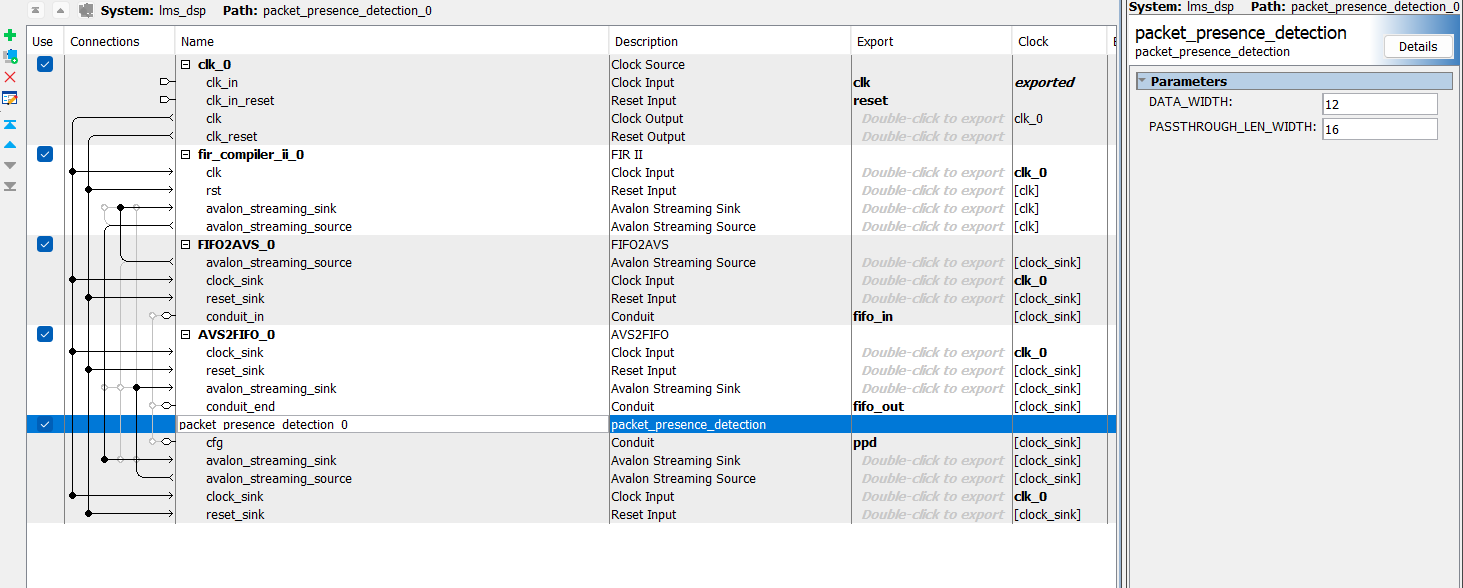
\includegraphics[width=\linewidth]{figures/ppd_detect_qsys_config.PNG}
    \caption{SystemVerilog parameters of the packet presence detector in QSYS.}
    \label{fig:pd_hard_param}
\end{figure}

\begin{table}[!h]
\centering
\begin{tabular}{|p{0.36\linewidth}|p{0.48\linewidth}|p{0.08\linewidth}|}
\hline
Parameter & Description & Default value \\
\hline
\textsc{DATA\_WIDTH} & Bit width of the samples & 12 \\
\hline
\textsc{PASSTHROUGH\_LEN\_WIDTH} & Bit width of the configurable number of samples to pass-through once the threshold is reached & 16 \\
\hline
\end{tabular}
\caption{SystemVerilog parameters of the \texttt{preamble\_detector} IP}
\label{table:pd_hard_param}
\end{table}

\subsection{Configuration signals}
\begin{sloppypar}
Additionally, there are several configuration signals that can be changed during operation from GNU Radio for better flexibility. Those configuration signals are listed in Table \ref{table:pd_soft_param}, you can trace them in the VHDL code, they are coming from the \texttt{fpgacfg} module defined in \texttt{LimeSDR-Mini\_lms7\_lelec210x/src/spi/fpgacfg.vhd} and located in the design hierarchy at \texttt{lms7\_trx\_top/inst0\_nios\_cpu/cfg\_top\_inst1/fpgacfg\_inst0}, as shown in Figure \ref{fig:design_hier_fpgacfg}.
\end{sloppypar}

This module contains a RAM with 16-bit words that retains the configuration of various elements of the FPGA. We used available addresses to put our custom configuration, the address map is written in the repo README. There are default values assigned at reset for the memory bits (Figure \ref{fig:design_hier_fpgacfg}) but they can be changed with a write operation.

\begin{table}[!h]
\centering
\begin{tabular}{|p{0.22\linewidth}|p{0.25\linewidth}|p{0.34\linewidth}|p{0.08\linewidth}|}
\hline
Configuration signal & Description & Allowed values\\
\hline
\texttt{cfg\_enable} & Enable or disable the PPD. & $\left\{0,1\right\}$ \\
\hline
\texttt{cfg\_clear\_} & Clear the delay lines of the dual running sum. & $\left\{0,1\right\}$ \\
\hline
\texttt{cfg\_PASSTHROUGH\_LEN} & Number of samples to pass-through after a start flag has been added. Avoid any retriggering of this flag meanwhile. & $\left[1,2^{\textsc{PASSTHROUGH\_LEN\_WIDTH}}-1\right]$ \\
\hline
\texttt{cfg\_THRESHOLD} & Value to multiply the normalized result of the long-term sum, before comparison. & $\left[1,2^{8}-1\right]$ \\
\hline
\end{tabular}
\caption{Configuration signals \texttt{packet\_presence\_detection} IP}
\label{table:pd_soft_param}
\end{table}

\begin{figure}[!h]
    \centering
    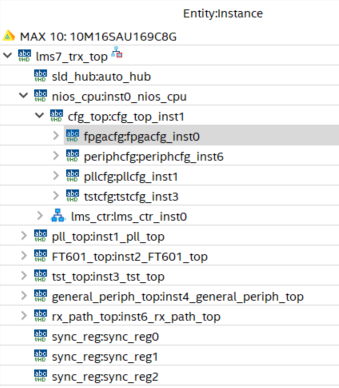
\includegraphics[width=0.3\linewidth]{figures/design_hierarchy_fpgacfg.PNG}
    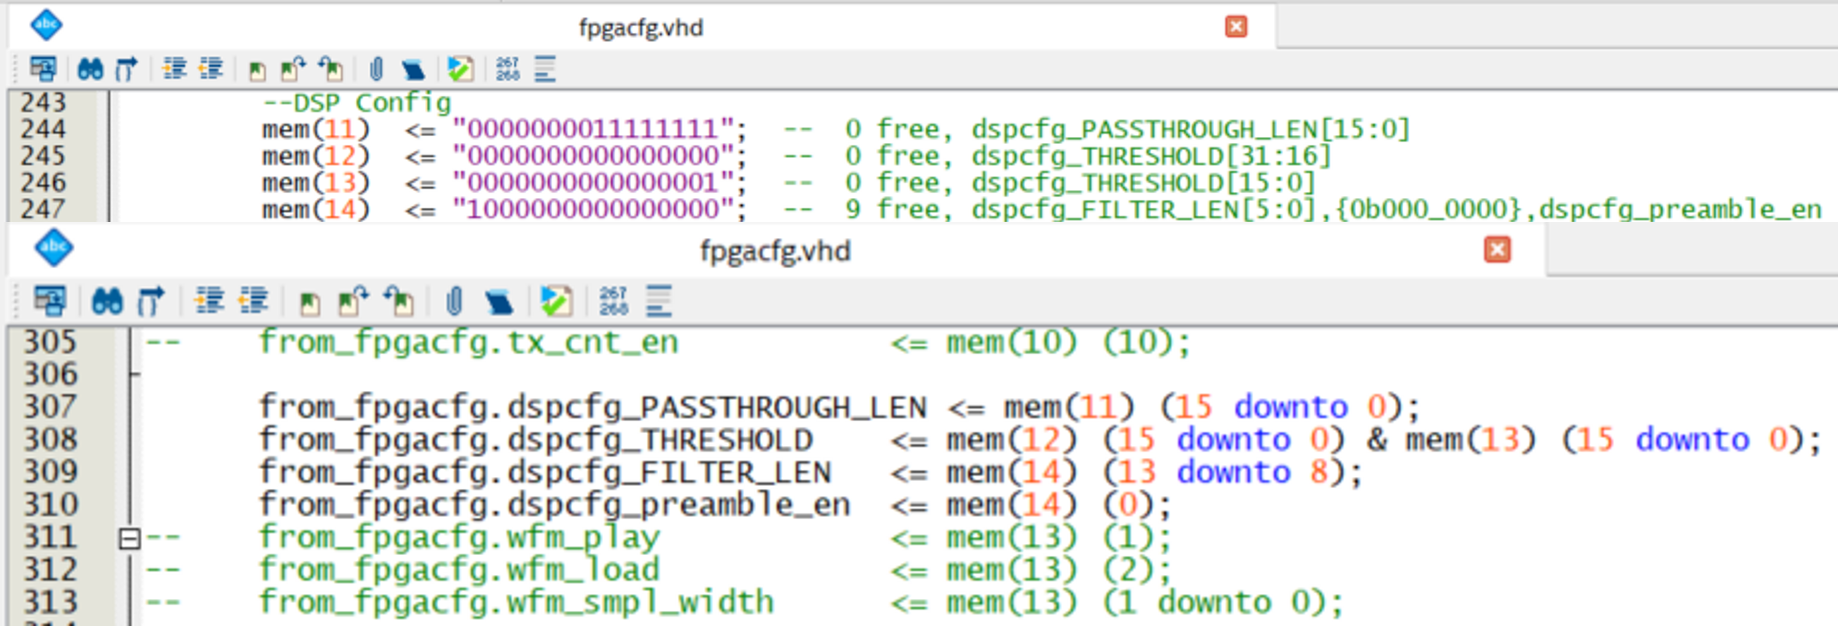
\includegraphics[width=0.6\linewidth]{figures/design_hierarchy_fpgacfg_both.PNG}
    \caption{Configuration signal location in the design hierarchy (left). Assignment and reset values for the DSP configuration signals (right).}
    \label{fig:design_hier_fpgacfg}
\end{figure}

\subsubsection{Read/write operations of the configuration signals from GNU Radio}
The GNU Radio block of the LimeSDR-Mini uses a C++ library called \textit{LimeSuite} in order to write data to the FPGA configuration memory. In the following paragraph, the configuration flow inside LimeSuite and the hardware is briefly described.

\begin{sloppypar}
\paragraph{gr-limesdr GUI interface}
In our custom version of the limeSDR GNU Radio block, we added fields to configure the hardware preamble detector. To do so, we modified the file \texttt{gr-limesdr/grc/limesdr\_fpga\_source.block.yml} and added a GUI callback function named \texttt{set\_dspcfg\_preamble}. This function is in turn defined in \texttt{gr-limesdr/lib/source\_impl.cc} and \texttt{gr-limesdr/lib/device\_handler.cc}. Please take a look at the end of \texttt{device\_handler.cc} and understand the functions we added. At the core of all of them, we use \texttt{modify\_spi\_reg\_bits}, shown in Figure \ref{fig:modify_spi_reg_bits}, that uses LimeSuite \texttt{LMS\_WriteFPGAReg} function. Pay attention to the arguments and try to make the link with the configuration memory of the FPGA, the input structures are defined in \texttt{gr-limesdr/lib/fpga\_register\_map.h}.
\end{sloppypar}

\begin{figure}[!h]
    \centering
    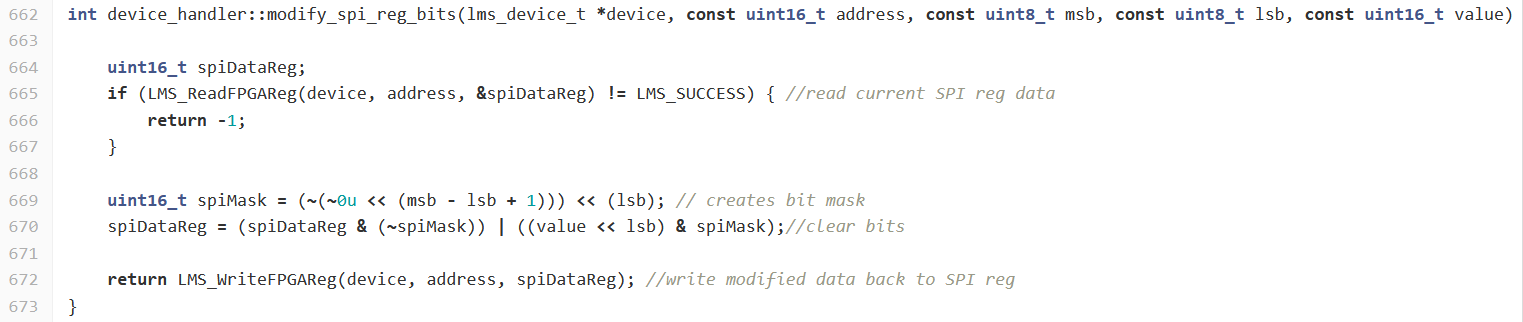
\includegraphics[width=\linewidth]{figures/grlimesdr_write_fpgacfg.PNG}
    \caption{Software interface between GNU Radio and LimeSuite.}
    \label{fig:modify_spi_reg_bits}
\end{figure}

\paragraph{NIOS Interface}
When calling \texttt{LMS\_WriteFPGAReg}, the functions wrap the address and value of the register we wish to configure inside a packet that is transmitted through USB. The complete callstack inside the library is described in the repo README. The USB interface is connected to an FTDI Chip which is in turn interfaced with the FPGA, as shown in Figure \ref{fig:limesdr_mini_schematic}.

Inside the FPGA, we have:
\begin{enumerate}
    \item An FTDI arbitrer that decodes a first part of the packet header to forward it through a configuration FIFO (\texttt{EP02\_fifo}) towards the NIOS subsystem. This arbitration is necessary as we have two other FIFOs coming from the NIOS subsystem and the RX data path (\texttt{EP83\_fifo} and \texttt{EP82\_fifo} respectively).
    \item A NIOS Softcore processor instantiated inside the FPGA reads the FIFO and decodes the second part of the packet header, it then forwards the packet data to through an SPI Master.
    \item An SPI Slave is connected with the configuration memory and writes the received data at the correct address.
\end{enumerate}

\begin{bclogo}[couleur = gray!20, arrondi = 0.2, logo=\bcinfo]{Additional resources}
To help you understand this complex path, we provided you with resources you can find on moodle or \texttt{LimeSDR-Mini\_lms7\_lelec210x/doc/} folder. The file \texttt{FPGA\_config\_path.pdf} with annotations referring to the above paragraph should be helpful, several elements have been hidden to ease the reading. You can also use freely the RTL viewer to skim through the design hierarchy graphically instead of opening files, see Figure \ref{fig:rtl_viewer} for further details.
\end{bclogo}

\begin{figure}[!h]
    \centering
    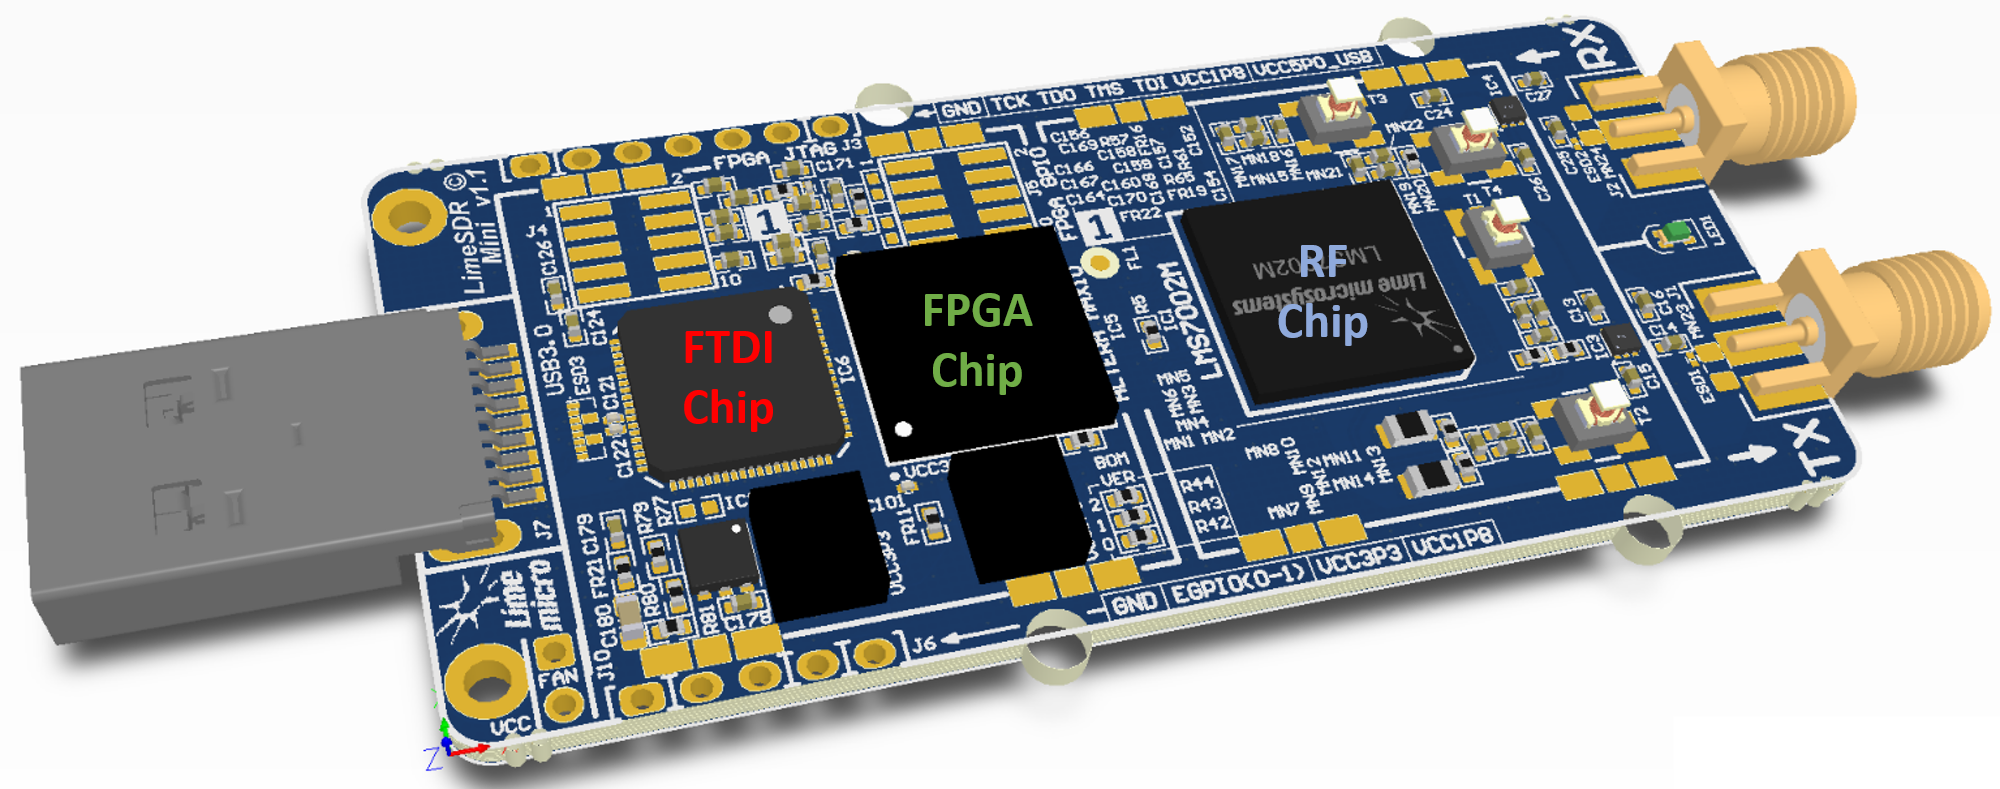
\includegraphics[width=0.7\linewidth]{figures/limesdrmini_schematic.png}
    \caption{Location of the different chips on the LimeSDR-Mini board.}
    \label{fig:limesdr_mini_schematic}
\end{figure}

\begin{figure}[!h]
    \centering
    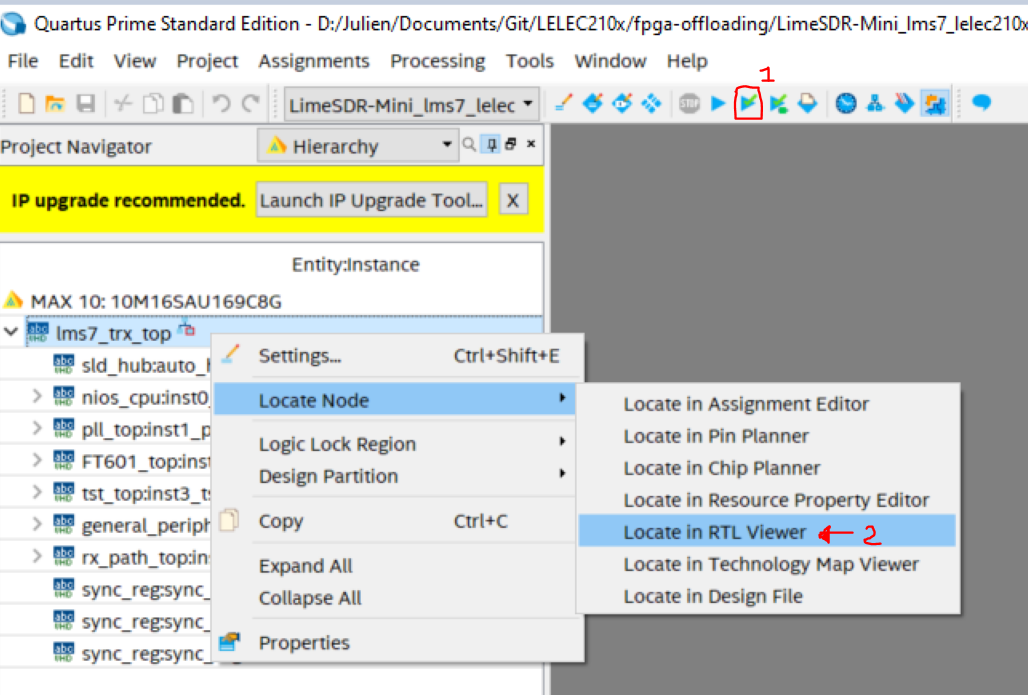
\includegraphics[width=0.7\linewidth]{figures/rtl_viewer.png}
    \caption{In order to use the RTL viewer, first elaborate the design (1) then right click on the design element you want view (2).}
    \label{fig:rtl_viewer}
\end{figure}




\end{document}
%%%%%%%%%%%%%%%%%%%%%%%%%%%%%%%%%%%%%%%%%%%%%%%%%%%%%%%%%%%%%%%%%%%%%%%%%%%%
